\section{Results}

\subsection{Idea Forest}

Hierarchical clustering yielded an idea forest composed of 3007 instances, 1213 unique ideas, 335 category trees, and 129 non-singleton category trees (Table~\ref{tab:idea_forest}). In general, category trees were shallow, with a maximum tree height of 5. The number of nodes within a category tree ranged from 1 to 66, with the distribution of values roughly following a Poisson distribution. The number of instances per node (i.e., the number of equivalent idea instances) also roughly follows a Poisson distribution, with number of instances ranging from 1 to 63.
\begin{table}
	\begin{tabular}[h!]{r | l l l l l l l}
	\textbf{number condition} & 5 & 10 & 20 & 50 \\ \hline \hline
	HITs & 57 & 47 & 23 & 10\\
	instances & 293 & 471 & 453 & 500 \\
	ideas & 171 & 249 & 278 & 341 \\
	category trees & 72 & 79 & 93 & 114 \\
	non-singleton trees & 28 & 34 & 40 & 48 \\ \hline \hline
	\textbf{number condition} & 75 & 100 & all \\ \hline \hline
    HITs & 10 & 10 & 146\\
	instances & 634 & 855 & 3007\\
	ideas & 443 & 177 &1212\\
	category trees & 172 & 177 &321\\
	non-singleton trees & 49 & 61 &92\\ 
	\end{tabular}
    \caption{Result counts between conditions}
    \label{tab:idea_forest}
\end{table}

% are also roughly poisson distributed (Table TAB). In keeping with the findings for height, trees found in the upper number conditions are smaller than trees found in the lower conditions. The precipitous drop in median tree size suggests that in the largest condition, participants are finding rare ideas with only a few variants and less than 14 instances.

% \begin{table}
% \begin{tabular}[h!]{r | l l l l l l l}
% 	\textbf{number condition} & 5 & 10 & 20 & 50 & 75 & 100 & all \\ \hline \hline
% 	number of nodes& \\ \hline
%     median &5&5&4&3&2&2&2 \\
% 	first quartile &2&2&1&1&1&1&1 \\
% 	third quartile &17&17&14&10&5&5&5 \\
% 	number of instances& \\ \hline
% 	median &14&14&12&10&4&4&4 \\
%     first quartile &4&4&4&2&1&1&1 \\
% 	third quartile &47&45&30&23&13&13&13 \\
% 	\end{tabular}
% 	\caption{Number of ideas and instances in trees}
% \end{table}

% \begin{figure}[h!]
%     \centering
%     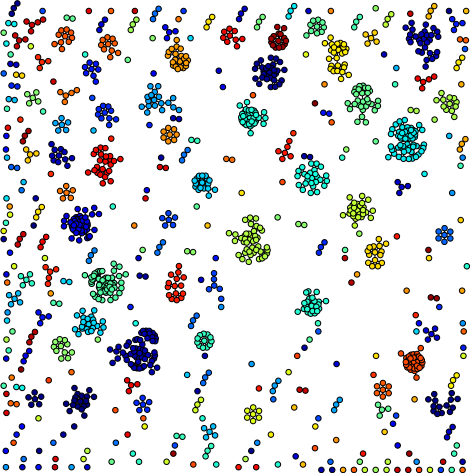
\includegraphics[width=0.9\columnwidth]{idea_forest}
%     \caption{Idea Forest}
% \end{figure}

% The height of category trees follows a roughly Poisson distribution, with the maximum tree height observed at 5. Summary statistics across condition are in table TAB. The third quartile drops as the number condition increases. While the upper conditions still discover categories trees with heights as great as 5, they generate many more "short" trees. This suggests that the ideas generated in the upper conditions are less common.

% \begin{table}
% 	\begin{tabular}[h!]{r | l l l l l l l}
% 	\textbf{number condition} & 5 & 10 & 20 & 50 & 75 & 100 & all \\ \hline \hline
% 	median & 2 & 2 & 2 & 2 & 2 & 2 & 2\\
% 	first quartile & 2 & 2  & 1 & 1 & 1 & 1 & 1\\
% 	third quartile & 3 & 3 &3 &3 &2 &2 & 2\\
% 	\end{tabular}
% 	\caption{Category tree height}
% \end{table}

\subsection{Rates of Idea and Category Production}
The idea forest allows us to model the rate at which new ideas and new categories of ideas are produced, testing hypotheses 1 and 2 (i.e., the notion that rates of new ideas and categories of ideas will diminish over time, and will do so as a function condition).

Figure FIG shows the cumulative count of new ideas as a function of the number of instances gathered in the experiment. For reference, a perfect ``1:1'' idea generation line is also plotted.

We model this quantity using the following logarithmic model:
\[n_{ideas} = b_0 + b_{cond} * \log (x_{scale} * x + x_{offset})\]
where $n_{ideas}$ represents the number of new ideas, $b_0$, $x_{scale}$, and $x_{offset}$ are parameters shared between conditions that serve to position the curve, and $b_{cond}$ acts as a per-condition scaling factor. This model does not explicitly model variability due to different workers, a point we return to later.

We fit the parameters to the data using a Bayesian approach [REF Kruschke], using the STAN modeling software to perform the actual fit [REF STAN]. In modeling the parameters, we use uninformative priors. The resulting posterior distributions allow us to determine whether the conditions are significantly different from one another by determining whether the highest density intervals (HDIs) of $b_{cond}$'s posterior distributions overlap or not. In our analyses, we use an HDI of 95\%.

Analysis of the HDIs of $b_{cond}$ reveals no significant differences between the 5 and 10 conditions, with all other conditions significantly different from one another except for the 50 and 100 conditions. [TODO: Table of fitted values and their HDIs.] Notable in our data is the 75 condition, which rises above the 100 condition in this plot. Further analysis reveals that a single worker is responsible for that additional rise in number of new ideas. Removing that worker from the data reveals that the 75 condition is not different from either the 50 or 100 conditions.

Taking the derivative of the models allows us to examine the same data, but as rates at which new ideas are produced. As expected, rates of new ideas quickly taper off as a function of the number of ideas received.

\begin{figure}[h!]
    \centering
    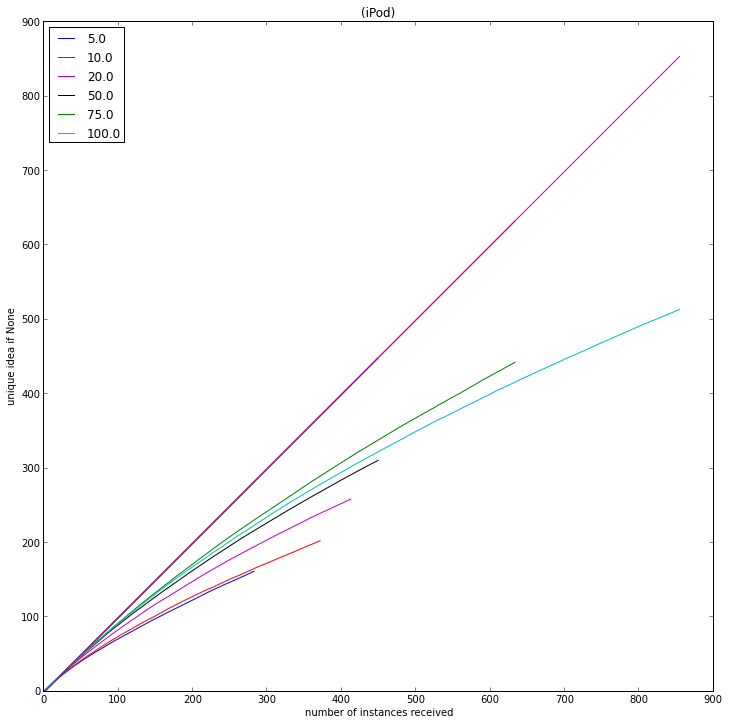
\includegraphics[width=0.9\columnwidth]{ideas_over_time}
    \caption{Cumulative idea count}
\end{figure}

\begin{figure}[h!]
    \centering
    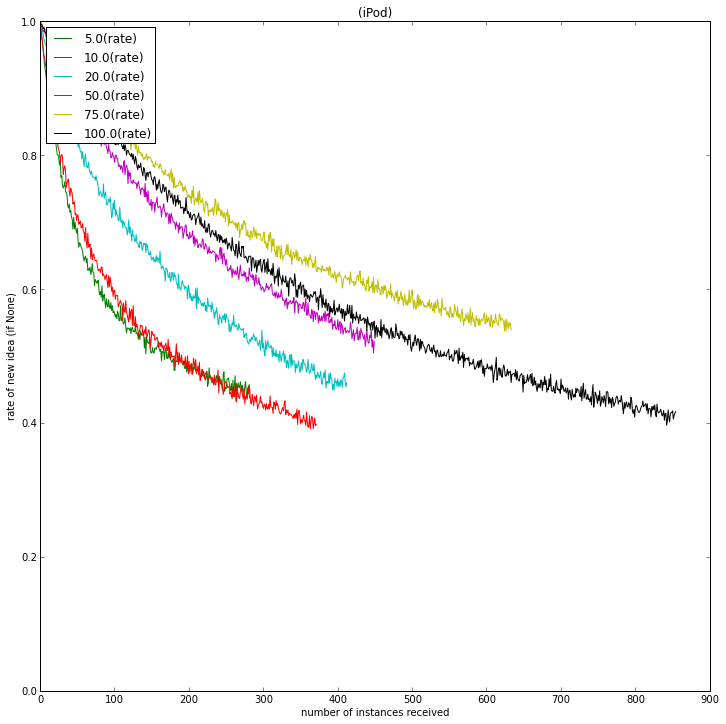
\includegraphics[width=0.7\columnwidth]{rate_new_idea_over_time}
    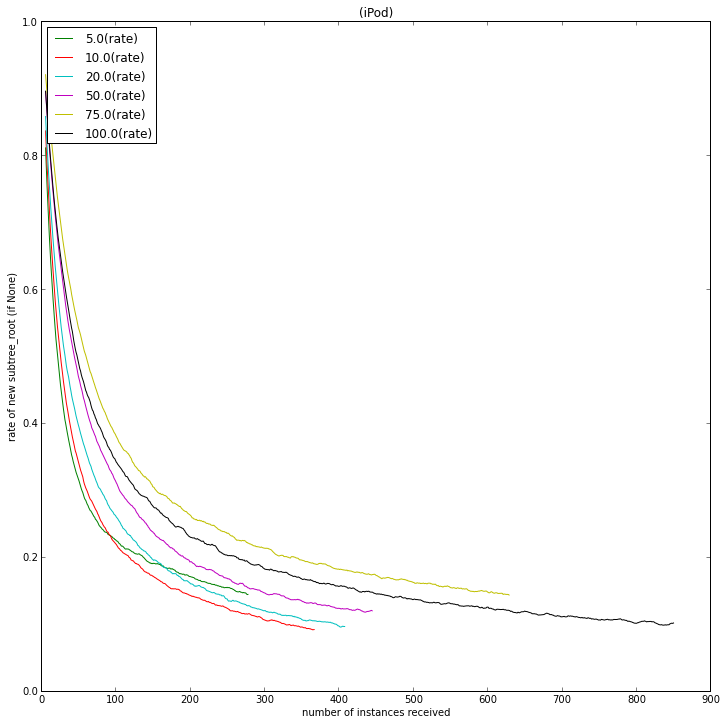
\includegraphics[width=0.7\columnwidth]{rate_new_category_over_time}
    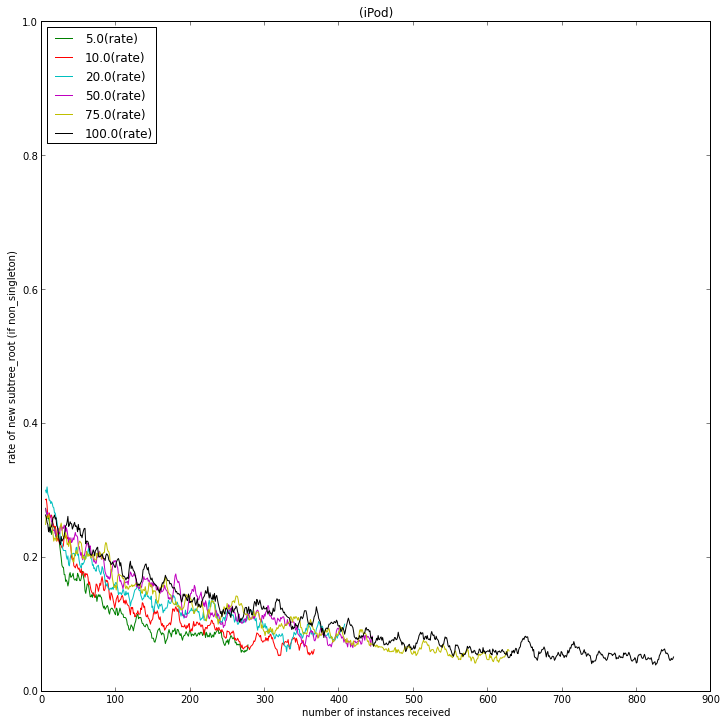
\includegraphics[width=0.7\columnwidth]{rate_new_ns_category_over_time}
    \caption{Rate of idea generation}
\end{figure}

We can perform a similar analysis for the number of new idea categories that arrive over time. As would be surmised from the previous graphs, we observe a similar pattern, which can also be modeled using a logarithmic model. In the fitted model, we see that the number of new idea categories produced increases more slowly than the number of new ideas. This finding suggests that although individuals may produce new, unique ideas over time, these new ideas are within the \emph{same} categories. In other words, they are ``riffing'' -- coming up with permutations on existing ideas.

Collectively, these results largely affirm hypotheses 1 and 2: The rates of new idea and new idea categories production quickly taper off and tend toward zero over time. Furthermore, we see differences in rates between conditions. In our data, we see three clear groups of rates: the 5 and 10 conditions, the 20 condition, and the 50, 75, and 100 condition.

%Given the observed differences in production of new ideas and idea categories, it is worthwhile to better understand \emph{why} these differences exist. 

%The third panel, which shows non-singleton categories over time, tells a distinctly different story from the others. While in the idea and category plots, the height-ordering of rates of generation between categories remains generally identical, there is a point of intersection and reversal in the non-singleton category plot at around the 30 instances point. Before this point, the lower conditions actually generate new categories at a \emph{faster} rate.

\subsection{Characteristics of an Idea Within a Run}
We now turn our attention to individual runs, and characterize the ideas produced throughout a run.

\subsubsection{Most Popular Ideas}
Our results suggest that individuals typically produce ideas from a common set idea categories early in the brainstorming process, then diverge and produce more original ideas. This phenomenon can be observed by examining the o-scores of ideas and idea categories in Figures X and Y, which show the distribution of o-scores for individual ideas and idea categories, as a function of response number, across all conditions.

%As our measure of originality, we use \emph{o-score}, introduced by Jansson and Smith \cite{jansson_design_1991}. An idea's o-score is $1 - p(idea)$, where $p(idea) = (number of instances of that idea)/(number of instances total)$. The o-score for category trees is similarly calculated. We will occasionally refer to the \emph{category o-score} of an idea. This simply refers to the o-score of the category tree to which that idea belongs.

% We measure differences in originality between conditions by examining the idea o-score and category o-score. The distributions of these scores are summarized in Figure FIG. The left panel compares idea o-score and the right compares category o-score.

%. Beyond the inflection point, the category pool is saturated with these low-hanging fruit, and only brainstormers tasked with generating more ideas will find the smaller category. This is a more nuanced view of the tree node/instance quartiles in Section SEC; condition 5 brainstormers cover the spectrum of category sizes while condition 100 brainstormers pull from the smaller category trees in the forest.



% The final measure, \emph{look-back equality}, is non-symmetrical and has meaning only in the context of a single brainstorming run. An instance \emph{a} is look-back equal to an \emph{earlier} instance \emph{b} if \emph{b} is in either \emph{a}'s idea node or any of \emph{a}'s parents, siblings, or children. This definition specifically identifies when a later instance in a run can be considered to have been influenced by earlier instance.



% \begin{figure}[h!]
%     \centering
%     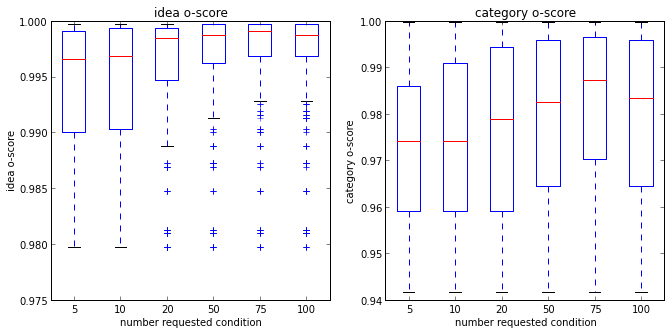
\includegraphics[width=0.9\columnwidth]{oscores_conditions}
% \end{figure}

% The more ideas requested, the more original the ideas produced. As suggested by the instance quartile range in section SEC, higher number conditions produce idea in trees with fewer instances, thus the high category o-score. We also see that these conditions produce \emph{ideas} with fewer instances.

% As the originality rises, however, so does the number of outliers. To understand this phenomenon, we need to more closely observe the distribution of originality scores between not just conditions, but ordinal position in a brianstorming run.

% Figure FIG provides this visualization. The upper panel gives the mean idea o-score as a function of ordinal position in all 100 condition brainstorming runs. The o-score for each ordinal position is the mean of all idea o-scores for that ordinal position in a run. Following this, the plot is further smoothed by making each point the mean of a sliding window of size 10 around its ordinal position. The bottom panel is a similar plot for category-oscore. To aid in interpretation, the first, second and third quartiles are also represented on the plot. The error bars are standard error.

% \begin{figure}[h]
%     \centering
%     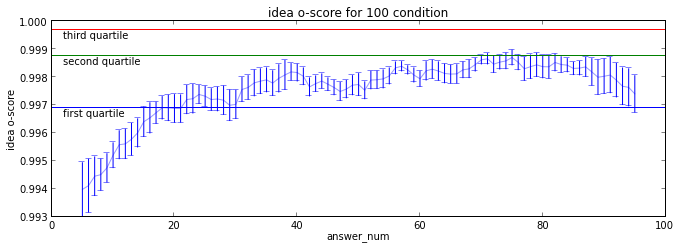
\includegraphics[width=0.9\columnwidth]{idea_oscore_order_100}
%     \caption{Idea o-score as a function of order (100 condition)}
%     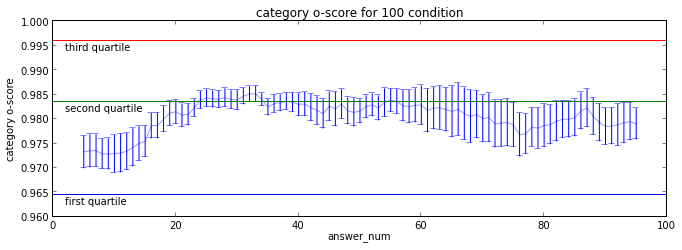
\includegraphics[width=0.9\columnwidth]{cat_oscore_order_100}
%     \caption{Category o-score as a function of order (100 condition)}
% \end{figure}

% The only part of the originality score that falls outside the first and third quartiles is the beginning of the run. Participants in the higher numbered conditions generate more original ideas overall, but not until they have exceeded some threshold of common ideas. Figure FIG replicates figure FIG but across all conditions, and the same pattern of originality growth until an originality peak - around 20 ideas - is reached. Note that because of the additional HITs, there are far more examples of early-order ideas in the 5, 10 and 20 conditions than in the 50, 75, or 100, so this pattern is present without any dominating affect by the upper conditions.

\begin{figure}[h]
    \centering
    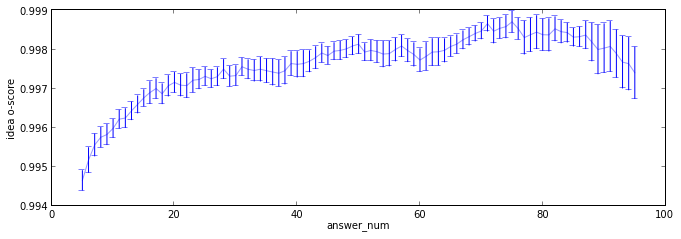
\includegraphics[width=0.9\columnwidth]{idea_oscore_order}
    \caption{Idea o-score as a function of response number, all conditions}
    \label{fig:idea_oscore_order}
    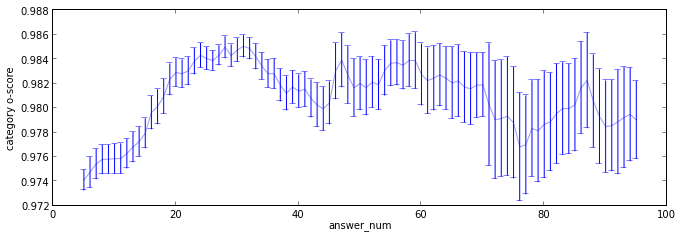
\includegraphics[width=0.9\columnwidth]{cat_oscore_order}
    \caption{Category o-score as a function of response number, all conditions}
    \label{fig:cat_oscore_order}
\end{figure}

In both instances, we observe a steady increase in o-scores for the first 20-30 responses. After these first 20-30 responses, the o-scores essentially plateau, with no clear discernible pattern for either ideas or idea categories.

These graphs lend support for hypothesis 3, the notion that there is a set of general, common ideas that make up the first several responses of every crowd brainstorming session, regardless of condition.

To more explicitly confirm this hypothesis, we extracted the top 5\% most common ideas (66 in total). If our intuition is correct, these ideas should be more likely to appear in the first five instances of a run than they are to appear in any of the following instances. We introduce two Bernoulli random variables to model this. The first, defined by parameter $\theta_f$ represents the probability that a response instance is in the top 5\% most common ideas, given it is found in the first five instances of a run ($P(\theta_f|top)$). The second, defined by parameter $\theta_l$, is the probability that an instance is in the common pool given it is one of the \emph{last} (>5) instances in a run ($P(\theta_l|top)$).

We fit these parameters using data from all runs that have more than 10 responses. We chose this constraint so that no run could contribute evidence to $\theta_f$ without also contributing to $\theta_l$. The resulting parameters were $\theta_f = 0.564$ (95\% HDI 0.517-0.611) and $\theta_l = 0.323$ (95\% HDI 0.303-0.342). This difference is significant, supporing the hypothesis that common ideas are over-represented in the early part of a brainstorming run.


%This is explained by the relationship between common ideas and common categories. We expect that unoriginal ideas belong to unoriginal categories, as a high instance count for an idea increases the instance count for its category tree. However, we cannot make the inverse assumption, that a high originality idea belongs to a high originality category. Once the common idea are exhausted, then, there is no relationship between idea originality and category originality.

\subsubsection{Hypothesis 4}
The steady increase in originality seen in the first 20 instances (Figure~\ref{fig:idea_oscore_order}, \ref{fig:cat_oscore_order}), provides evidence for \textbf{Hypothesis 4:} ideas generated in the second half a brainstorming session have higher o-scores than those in the first half.
With the point of change seen at the 20 point, we use this as our division point, fitting two each for idea and category o-scores: instances in the first 20 of runs, and instances in the second 20 runs.
In examining the data, it became clear that o-scores do not follow a remotely normal distribution. Instead, we fit a beta distributions to each data division. The results are in Table~\ref{tab:hyp4} and Figure~\ref{fig:idea_oscore_hyp4}.

\begin{table}
	\begin{tabular}[h!]{r | l l }
	    & $\alpha$ median & $\alpha$ 95\% HDI \\ \hline \hline
        idea o-score (\textless=20) & 135.86 & 122.39-149.72 \\
        idea o-score (\textgreater20) & 259.84 & 240.47-278.81 \\ \hline \hline
	    & $\beta$ median & $\beta$ 95\% HDI \\ \hline \hline
        category o-score (\textless=20) & 1.16 & 1.08-1.25 \\
        category o-score (\textgreater20) & 0.82 & 0.77-0.86 \\
	\end{tabular}
    \caption{Hypothesis 4 Beta models}
    \label{tab:hyp4}
\end{table}

\begin{figure}[h]
    \centering
    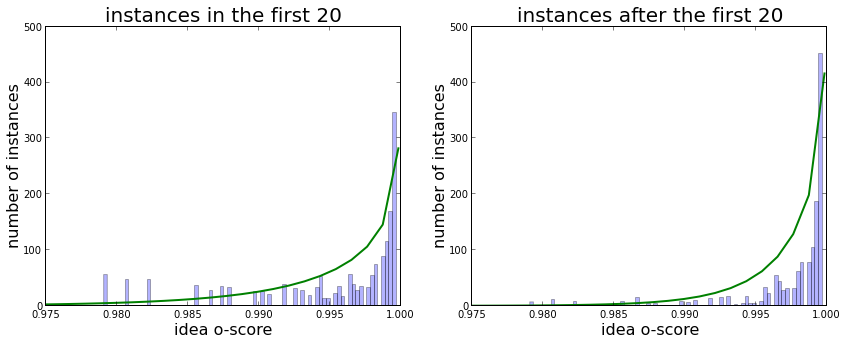
\includegraphics[width=0.9\columnwidth]{hyp4_ideas}
    \caption{Beta models for idea o-score}
    \label{fig:idea_oscore_hyp4}
    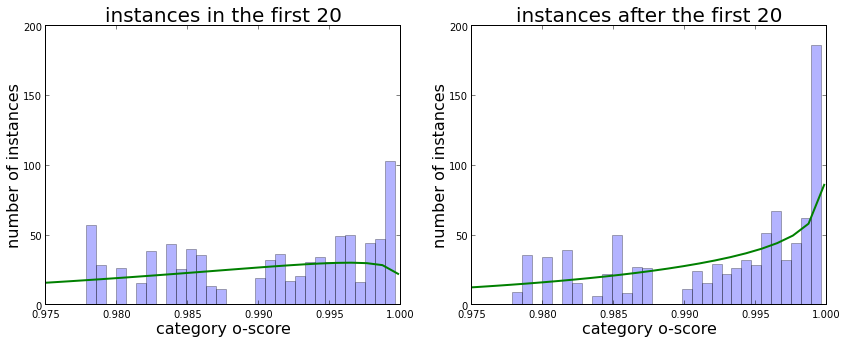
\includegraphics[width=0.9\columnwidth]{hyp4_cats}
    \caption{Beta models for category o-score}
    \label{fig:cat_oscore_hyp4}
\end{figure}

The idea o-score models are significantly different in the $\alpha$ parameter, with mean o-scores of 0.995 and 0.997 for the $\leq20$ and $\textgreater20$ conditions respectively. The category o-scores are significantly different in both parameters, with mean o-scores of 0.975 and 0.982.

Participants generated more original ideas after their first 20 instances than they did after. Not only does this support the hypothesis, it provides a clear guideline for maximizing originality in brainstorming tasks on microtask marketplaces: it is more cost-effective to solicit $\textgreater20$ ideas from a smaller pool of participants than to ask for less from more.




\subsection{Idea Generation Patterns}
Given the clear differences in characteristics of ideas as a function of response number, we now consider idea generation patterns observable from the data. In this section, we examine these patterns in the context of hypotheses 5 and 6. Specifically, these hypotheses draw upon the SIAM model and predict that individuals will generate ideas from an idea category until they exhaust that category, at which point they switch to another category (hypothesis 5). Furthermore, SIAM predicts that this category switching will be observable as taking more time to generate an idea in a new category than in the existing category (hypothesis 6).

To determine category switching, we examine whether an idea was assigned to the same category tree as the previous, or whether it was assigned to a different category tree. We also examine the timing data collected from the web app to examine the time to generate an idea as a function of whether it is in the same category as the previous idea.

Our data show clear evidence in support of both hypotheses. As an example, below is an example of a worker riffing on a single idea.

%An example of a single participant's riffed responses is given in Figure FIG. The second column is dark if the response instance is a permutation of any idea earlier in the run. The first column is dark if the instance is a \emph{source} instance, meaning it is the source for later permutations. Permutation chains can either be consecutive (as in this example), or separated with instances in between. The third column simply provides the text for that instance.

% \begin{figure}[h]
%     \centering
%     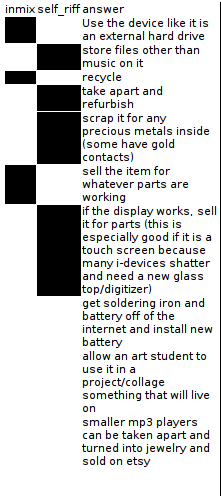
\includegraphics[width=0.5\columnwidth]{10_riff}
%     \caption{Example of riffing in a size 10 run}
% \end{figure}

%The participant hits on the categories of using the device's hard drive for storage, recycling the device or its materials, and selling the device.  within these categories, they generate 2-3 ideas each. This is a fairly typical example of riffing. In larger conditions, it is common for participants to reach further back and return to an idea multiple time. Table TAB provides a summary of riffing between conditions.

\begin{table}
\begin{tabular}[h!]{r | l l l l l l l}
    \hline \hline \textbf{condition} & 5 & 10 & 20  \\ \hline \hline
    \% riffs & 13.65 & 19.28 & 25.17  \\
    source instances & 10.58 & 12.92 & 15.01 \\
    riffs per source & 1.29 & 1.49 & 1.68 \\
    median length of consecutive chain & 2 & 2 & 2 \\
    median distance to previous in chain & 1 & 2 & 2 \\
    median distance to first in chain & 2 & 3 & 5 \\ \hline \hline
    \textbf{condition} & 50 & 75 & 100 \\ \hline \hline
    \% riffs & 39.6 & 32.81 & 42.81 \\
    source instances & 19 & 17.19 & 18.13\\
    riffs per source & 2.08 & 1.91 & 2.36\\
    median length of consecutive chain & 2 & 2 & 2\\
    median distance to previous in chain & 7 & 10 & 5\\
    median distance to first in chain & 16.5 & 18 & 26.5 \\
    \end{tabular}
    \caption{Riffing statistics by condition}
\end{table}

Examining our data, we find that the higher the number of instances requested, the more likely participants are to use old ideas as inspiration for new ideas (i.e., ``riff'' on previous ideas). However, these riff sequences are typically quite small in length, across conditions.

To explicitly test hypothesis 5, we model the probability of any idea category being followed by the same idea category with a Bernoulli random variable. Using a uniform beta prior, we find the probability of a response instance being in the same idea category as the previous to be 15.6\% (95\% HDI 14.3\% - 17.0\%). To establish a baseline to understand whether this probability is greater than chance, the most popular category tree in our data set is \emph{music player}, representing 5.65\% of all instances. Thus, the greatest probability of one instance being in the same category as the previous instance, by chance, is 5.65\%, well below the 14.3\% lower bound of the calculated HDI. Thus, we accept the hypothesis that an instance follows a previous instance in the same category with greater probability than is explained by random chance.

To test hypothesis 6, we now examine the time it takes to generate a response instance.

An examination of the distribution of data for time spent per instance suggests a log-normal distribution to the data. Using STAN, we fit two models: $t_w = \text{lognormal}(\mu_w, \sigma_w)$ for within-category idea generation and $t_b = \text{lognormal}(\mu_b, \sigma_b)$ for between-category idea generation, where the $t$ parameter in each model represents the time spent generating an instance.

\begin{figure}[h]
    \centering
    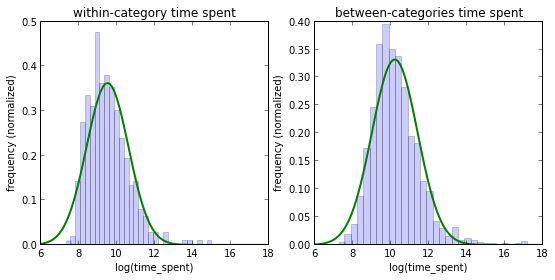
\includegraphics[width=0.9\columnwidth]{hyp5_comparison}
    \caption{Time spent to generate an instance}
\end{figure}

The resulting fit models are shown in Figure FIG, overlapping the log-space histograms for observed values. The mean for the within-category condition was 9.5 in log space (13.4 seconds, 95\% HDI 9.4-9.6), while the mean for the between-categories condition was 10.2 (27.0 seconds, 95\% HDI 10.2-10.3). The variances were 1.1 (3 seconds) and 1.2 (3.3 seconds) respectively. These difference were both sigificant. Within-category instance generation took on average 12.6 seconds less than between-categories. This is consistent with the findings of Nijstad and Stoebe, who reported differences of 6-12 seconds between conditions. Thus, we find support for hypothesis 6 and also show the applicability of the SIAM model to brainstorming in microtask marketplaces.

%Figure FIG displays the mean time spent on an instance by order, separated by condition. Most of the highly variant response times take place early in the brainstorming run. This suggests that at least one participant accepted a brainstorming task, took an initial stab at instances, and then left the task for up to 8 hours before continuing. Beyond this, we might expect to see time spent per instance go up as participants have to dig deeper to find responses, but no such effect is consistently observed.

% \begin{figure}[h]
%     \centering
%     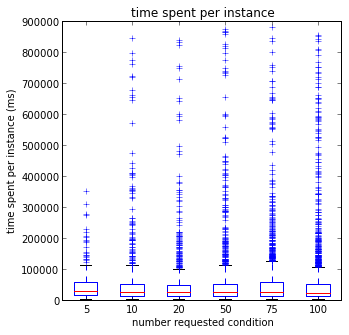
\includegraphics[width=0.9\columnwidth]{time_spent_condition}
%     \caption{Time spent per instance}
% \end{figure}


% \begin{figure}[h]
%     \centering
%     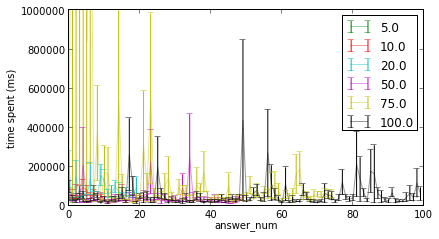
\includegraphics[width=0.9\columnwidth]{time_spent_order}
%     \caption{Time spent per instance}
% \end{figure}


%The Nijstad and Stroede \cite{nijstad_how_2006} model also provides \textbf{Hypothesis 5}: \emph{idea generation when changing semantic categories should take longer than idea generation within categories}. 

